\newpage

\section*{\centerline{Цель работы}}

Получение навыков работы с командной строкой UNIX и UNIX-подобных систем, а также навыки работы с файлами: просмотр редактирование, поиск и архивирование в GNU/Linux. Изучить основные команды и утилиты, поработать с правами на файлы и директории в GNU/LINUX. 
\newpage

\section*{\centerline{Выполнение}}
\vspace{1cm}

\subsection*{\centerline{Часть 1}}
\vspace{1cm}

Команда \textit{wget --spider url} позволяет проверить доступность файла по указанному адресу.\\
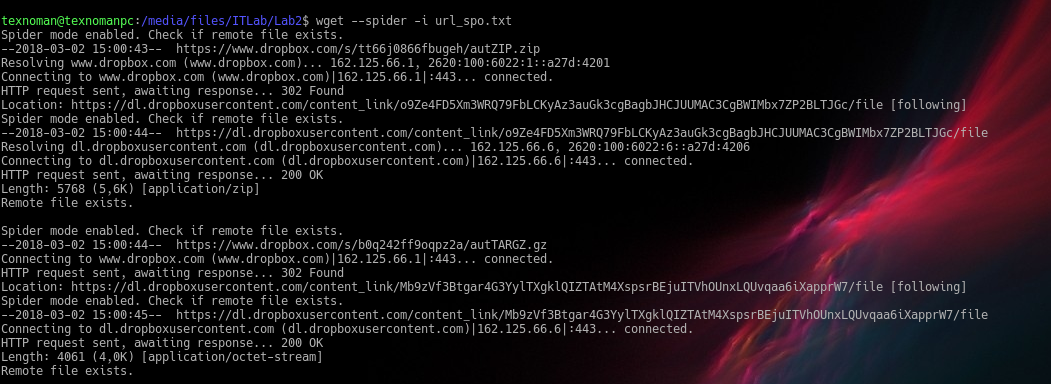
\includegraphics [width=\textwidth]{picture1.png}\\
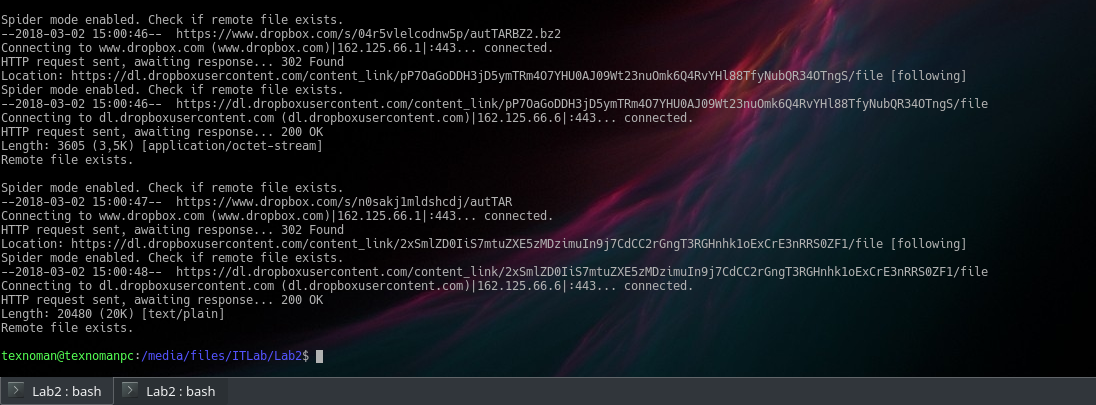
\includegraphics [width=\textwidth]{picture2.png}\\
\vspace{0.5cm}

Команда \textit{wget -i filename} позволяет перемещать и переименовывать файлы и папки.\\
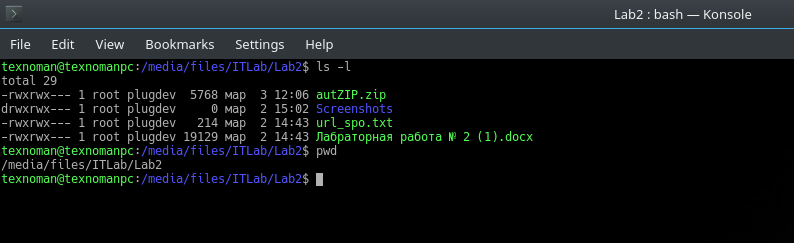
\includegraphics [width=\textwidth]{picture3.png}\\
\vspace{0.5cm}

Создание папки \textit{lab2} в домашней директории и Скачивание второго доступного файла\\
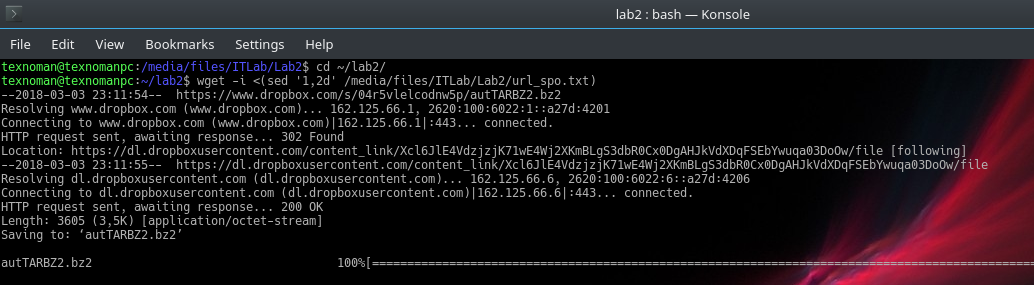
\includegraphics [width=\textwidth]{picture5.png}\\
\vspace{0.5cm}

Скачивание остальных файлов\\
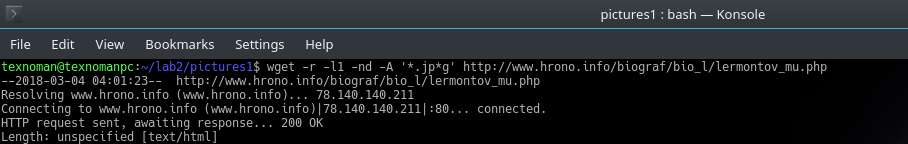
\includegraphics [width=\textwidth]{picture6.png}\\
\vspace{0.5cm}
